\documentclass{article}
\usepackage{amsmath}
\usepackage{graphicx}
\usepackage{booktabs}

\title{Analysis of Strategic Behavior in Two-Period School Choice Mechanisms with Switching Costs}
\author{HUANG XING}
\date{\today}

\begin{document}
\maketitle

\section{Results for 3 Students and 3 Schools Scenario}

In this section, I present my analysis of strategic behavior in a 3x3 school choice mechanism implemented over two rounds. My simulation framework systematically explores the possibility of beneficial preference manipulation.

\subsection{Simulation Framework}
My code implements a comprehensive search for strategic manipulation opportunities with the following structure:
\begin{itemize}
    \item Student $s_1$'s true preference is fixed as: $c_1 \succ c_2 \succ c_3 $
    \item For all other agents (2 students and 3 schools), each has 6 possible preference orderings
    \item This creates a total of $6^5=7776$ possible preference combinations to examine
\end{itemize}

\subsection{Strategic Analysis Methodology}
For each preference profile, I investigate whether $s_1$ can benefit from strategic manipulation through:
\begin{enumerate}
    \item First round: $s_1$ misreports preferences while others report truthfully
    \item Second round: 
        \begin{itemize}
            \item I examine all possible preference updates by other students in response to first-round outcomes
            \item $s_1$ reverts to truthful reporting
        \end{itemize}
    \item Comparison: I compare $s_1$'s final outcome under strategic behavior versus truthful reporting
\end{enumerate}

\subsection{Key Findings}
My exhaustive simulation revealed:
\begin{itemize}
    \item Among the $6^5$ total cases examined, 144 cases demonstrated successful strategic manipulation
    \item In these cases, $s_1$'s strategic misreporting in the first round, followed by truthful reporting in the second round, led to a strictly better outcome compared to being truthful throughout
    \item This suggests that even in a relatively simple two-round matching mechanism, there exist significant opportunities for beneficial strategic behavior
\end{itemize}

\subsection{Detailed Case Study of Beneficial Strategic Behavior}
Let's examine a specific case (Case ID 1044) that demonstrates how strategic manipulation can lead to better outcomes:

\begin{figure}[h]
\centering
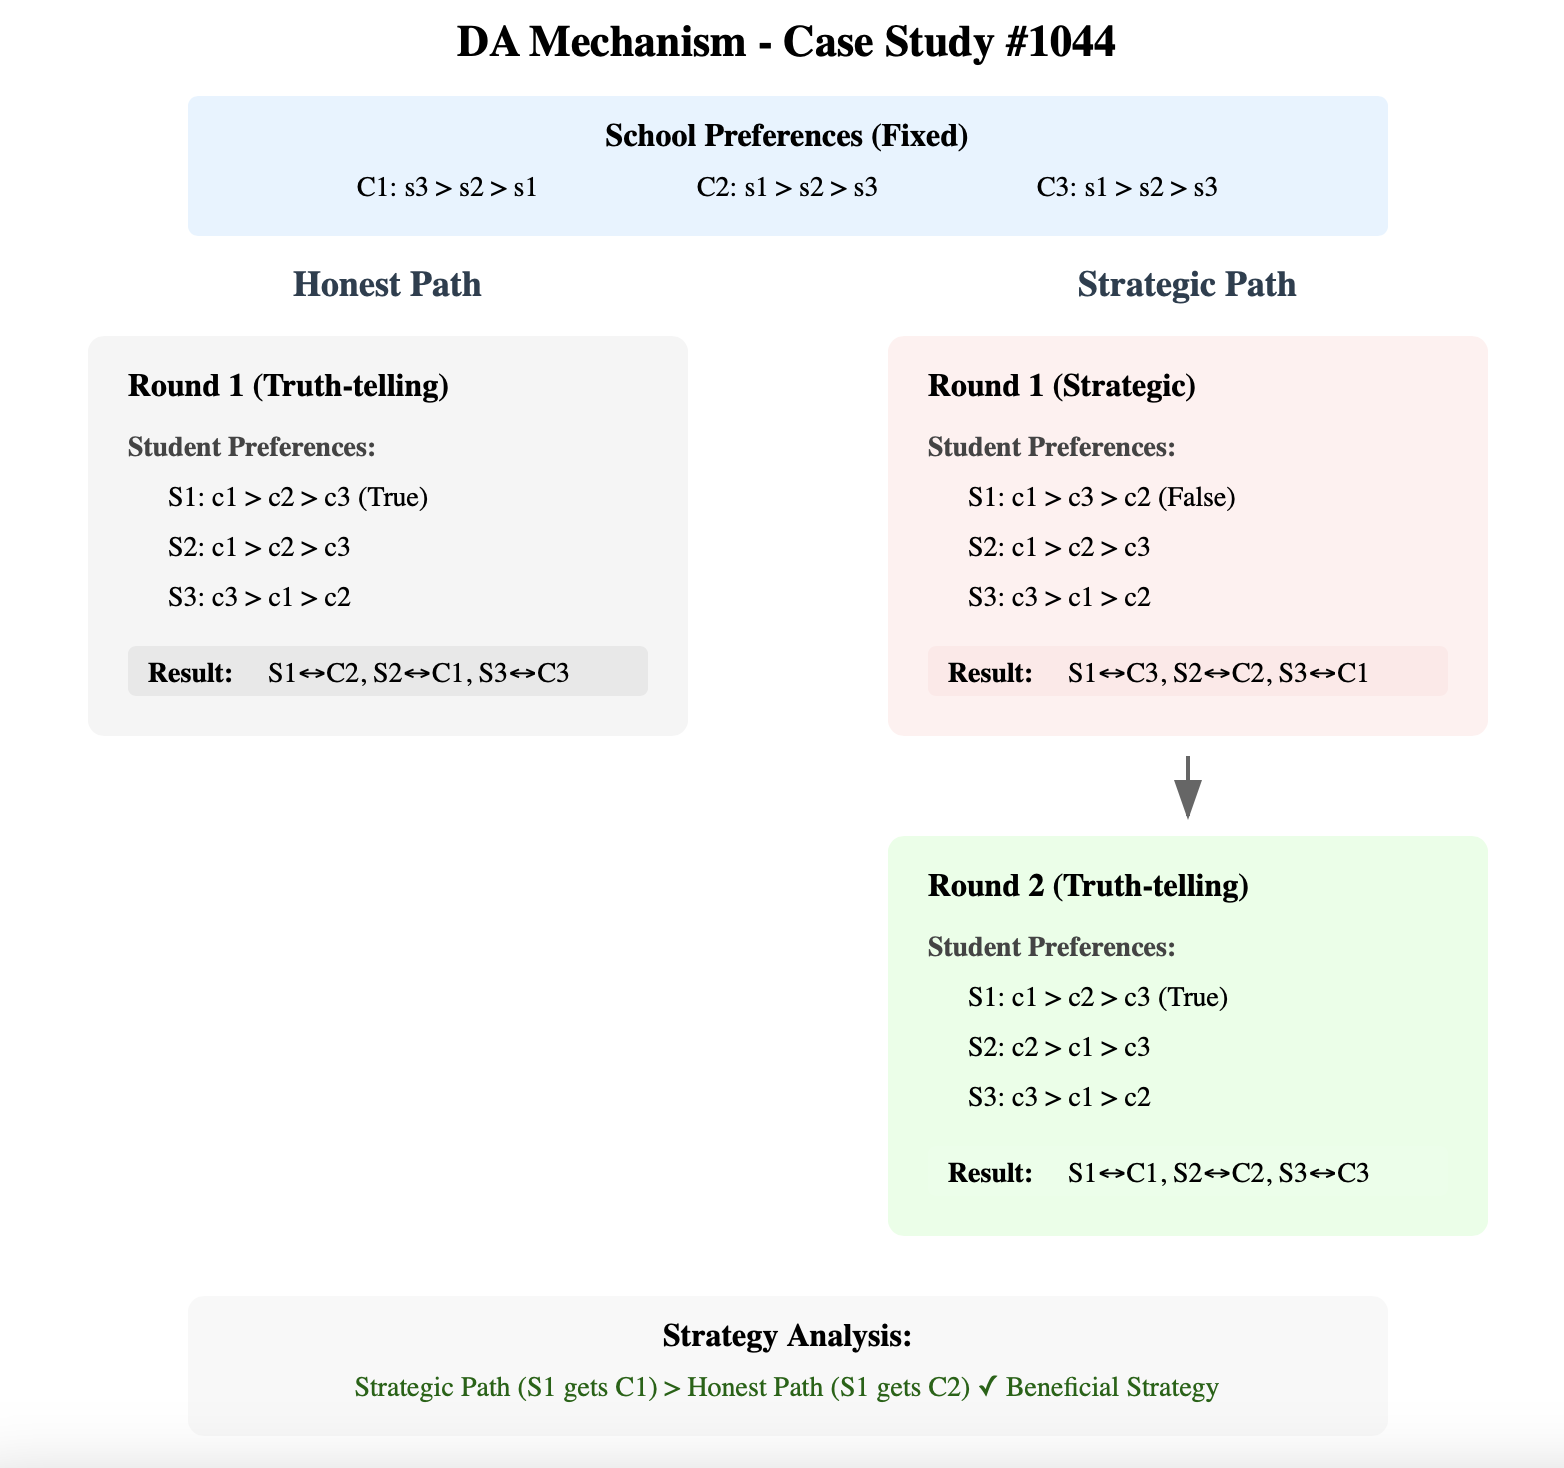
\includegraphics[width=0.7\textwidth]{3*3.png}
\caption{Strategic manipulation in 3x3 school choice mechanism}
\end{figure}

\subsubsection{Initial Preference Setup}
\begin{itemize}
    \item True Student Preferences:
    \begin{itemize}
        \item $s_1$: $c_1 \succ c_2 \succ c_3$
        \item $s_2$: $c_1 \succ c_2 \succ c_3$
        \item $s_3$: $c_3 \succ c_1 \succ c_2$
    \end{itemize}
    \item School Preferences:
    \begin{itemize}
        \item $c_1$: $s_3 \succ s_2 \succ s_1$
        \item $c_2$: $s_1 \succ s_2 \succ s_3$
        \item $c_3$: $s_1 \succ s_2 \succ s_3$
    \end{itemize}
\end{itemize}

\subsubsection{Truthful Reporting Scenario}
When all students report preferences honestly:
\begin{itemize}
    \item First round matching: $\mu_1 = \{(s_1,c_2), (s_2,c_1), (s_3,c_3)\}$
    \item $s_1$ receives second choice $c_2$
\end{itemize}

\subsubsection{Strategic Manipulation}
$s_1$ employs the following strategy:
\begin{enumerate}
    \item Misreports first-round preference as: $c_1 \succ c_3 \succ c_2$
    \item First round matching results: $\mu'_1 = \{(s_1,c_3), (s_2,c_2), (s_3,c_1)\}$
    \item Second round preference updates:
    \begin{itemize}
        \item $s_2$ updates to: $c_2 \succ c_1 \succ c_3$
        \item $s_3$ maintains: $c_3 \succ c_1 \succ c_2$
    \end{itemize}
    \item $s_1$ reverts to truthful reporting in second round
    \item Final matching: $\mu'_2 = \{(s_1,c_1), (s_2,c_2), (s_3,c_3)\}$
\end{enumerate}
Through this strategic manipulation, $s_1$ ultimately obtains their top choice $c_1$, a clear improvement over $c_2$ received under truthful reporting. 



\section{Results for 4 Students and 4 Schools Scenario}
For the expanded scenario with 4 students and 4 schools, the complexity increases significantly.\\
With 24 possible preference orderings per agent and 7 agents making choices (4 schools and 3 other students), there are $24^7$ (approximately 4.5 billion) possible combinations.\\
Due to this computational complexity, a sampling approach was employed to explore the strategy space.\\
Even with a limited sample size of 50 cases, instances where strategic manipulation remains beneficial were identified. Let's examine one such case (Case ID 13):
\begin{figure}[h]
\centering
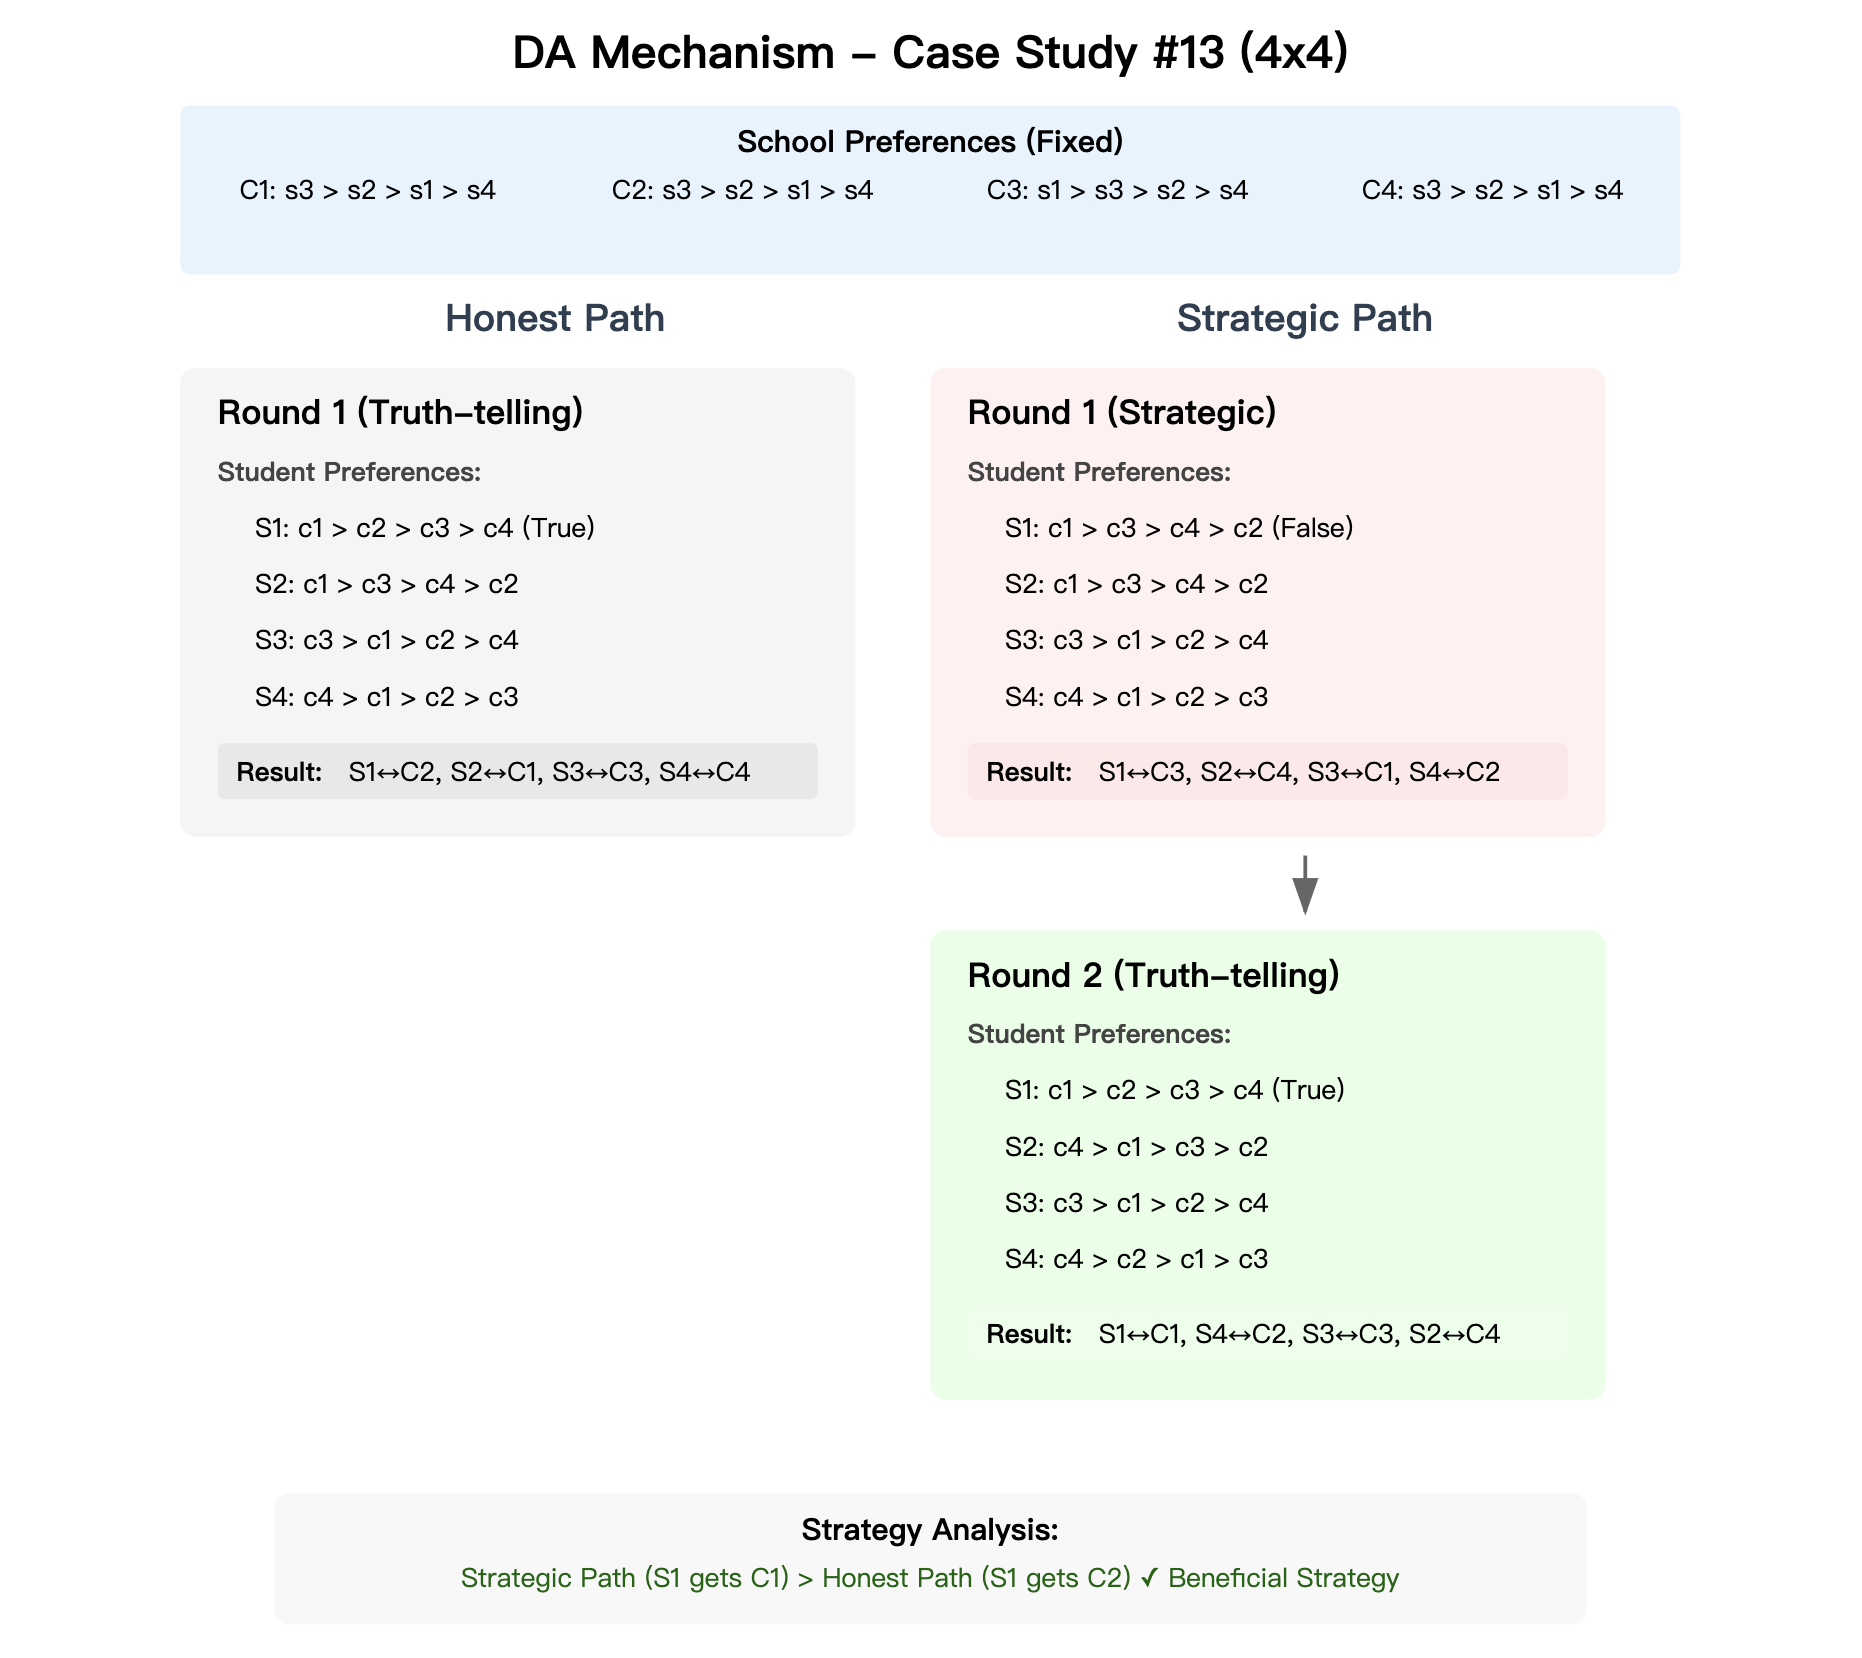
\includegraphics[width=0.7\textwidth]{4*4.png}
\caption{Strategic manipulation in 4x4 school choice mechanism}
\end{figure}


\subsection{Initial Preference Setup}
\begin{itemize}
    \item True Student Preferences:
    \begin{itemize}
        \item $s_1$: $c_1 \succ c_2 \succ c_3 \succ c_4$
        \item $s_2$: $c_1 \succ c_3 \succ c_4 \succ c_2$
        \item $s_3$: $c_3 \succ c_1 \succ c_2 \succ c_4$
        \item $s_4$: $c_4 \succ c_1 \succ c_2 \succ c_3$
    \end{itemize}
    \item School Preferences:
    \begin{itemize}
        \item $c_1$: $s_3 \succ s_2 \succ s_1 \succ s_4$
        \item $c_2$: $s_3 \succ s_2 \succ s_1 \succ s_4$
        \item $c_3$: $s_1 \succ s_3 \succ s_2 \succ s_4$
        \item $c_4$: $s_3 \succ s_2 \succ s_1 \succ s_4$
    \end{itemize}
\end{itemize}

\subsection{Successful Strategic Manipulation}
Under truthful reporting, student $s_1$ receives second choice $c_2$. However, by employing the following strategy:

\begin{enumerate}
    \item First round: Misreport preferences as $c_1 \succ c_3 \succ c_4 \succ c_2$
    \item This results in first-round matching: $\mu'_1 = \{(s_1,c_3), (s_2,c_4), (s_3,c_1), (s_4,c_2)\}$
    \item In the second round, after preference updates:
    \begin{itemize}
        \item $s_1$ reverts to true preferences: $c_1 \succ c_2 \succ c_3 \succ c_4$
        \item $s_2$ updates to: $c_4 \succ c_1 \succ c_3 \succ c_2$
        \item $s_3$ updates to: $c_3 \succ c_1 \succ c_2 \succ c_4$
        \item $s_4$ updates to: $c_4 \succ c_2 \succ c_1 \succ c_3$
    \end{itemize}
    \item Final matching: $\mu'_2 = \{(s_1,c_1), (s_4,c_2), (s_3,c_3), (s_2,c_4)\}$
\end{enumerate}
Through this manipulation, $s_1$ successfully obtains their first choice $c_1$ instead of their second choice $c_2$, demonstrating that beneficial strategic behavior persists even in larger matching markets.


\subsection{Alternative Pattern of Strategic Manipulation}
Another interesting pattern of strategic manipulation was observed in the simulation (Case ID 20):

\begin{figure}[h]
\centering
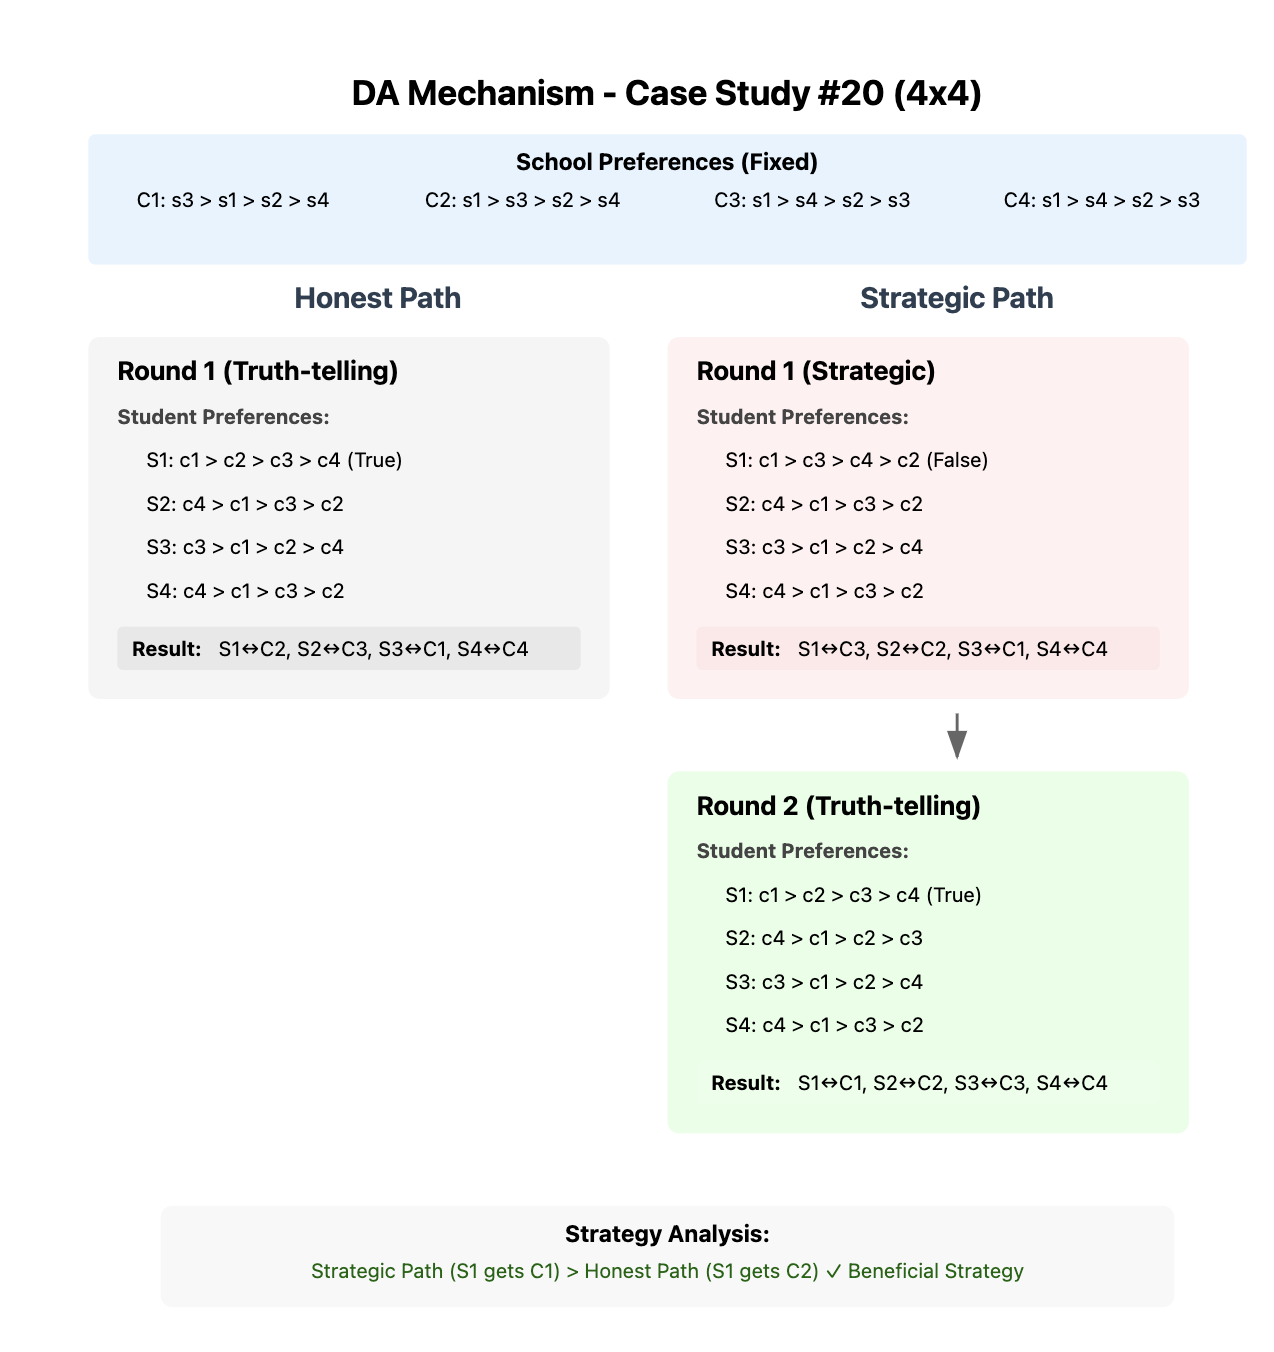
\includegraphics[width=0.7\textwidth]{4*4case2.png}
\caption{Alternative pattern of strategic manipulation in 4x4 school choice mechanism}
\end{figure}
In this case, student $s_1$ successfully manipulates by misreporting their preferences as $c_1 \succ c_3 \succ c_4 \succ c_2$ in the first round, which changes $s_2$'s matching outcome. This leads $s_2$ to no longer compete with $s_3$ for $c_3$ in the second round, which in turn causes $s_3$ to not compete with $s_1$ for $c_1$. Through this chain of reduced competition, $s_1$ is able to obtain their preferred school $c_1$ in the second round.


\section{Intuition Behind First-Round Manipulation}
The intuition behind successful first-round manipulation can be categorized into two main scenarios:

\subsection{Scenario 1: Weakening Direct Competition}
In this scenario, student $s_1$ with true preferences $c_1 \succ c_2 \succ c_3$ who receives $c_2$ under truthful reporting can benefit from strategic manipulation through the following mechanism:

\begin{itemize}
    \item First round: $s_1$ misreports to take $s''$'s target school, forcing $s''$ to compete for and obtain $s'$'s target school, which in turn forces $s'$ to match with a less preferred school $c'$
    \item Second round: If $s'$ develops a strong preference for $c'$ relative to $c_1$, they will no longer compete with $s_1$ for $c_1$
    \item This allows $s_1$ to obtain $c_1$ in the second round
\end{itemize}

For this strategy to work in a three-student setting:
\begin{itemize}
    \item $s_1$ must rank higher than $s''$ at $s''$'s target school
    \item At $c_1$, the preference order must be $s'' \succ s' \succ s_1$
    \item $s'$ must develop a strong second-round preference for their first-round match
    \item $s''$ should not develop a strong second-round preference for $c_1$
\end{itemize}
A natural question arises: would such strategic manipulation still be possible if schools have similar preferences over students (as is common in real-world labor markets where firms often value similar candidate qualities)? The answer is no - when schools have identical preferences over students, or when students have identical preferences over schools, such strategic manipulation becomes impossible. This is because the chain reactions and competition effects  rely fundamentally on the heterogeneity of preferences across both sides of the market.





\subsection{Scenario 2: Chain Reaction of Preference Changes}
The second scenario involves creating a chain reaction of matching changes:

\begin{itemize}
    \item $s_1$ manipulates to make competitor $s'$ obtain a better school $c'$ than $c_1$ in round two
    \item This can be achieved through two sub-scenarios:
    \begin{itemize}
        \item Sub-scenario 1: First-round manipulation changes the match of student $s''$ who competes with $s'$ for $c'$. If $s''$ develops a strong preference for their new match, they won't compete for $c'$ in round two
        \item Sub-scenario 2: Manipulation leads to $s''$ obtaining an even better school than $c'$ in round two, removing them from competition for $c'$
        \begin{itemize}
            \item This could trigger further chain reactions where $s''$ displaces another student $s'''$ from their match
            \item Student $s'''$ may then obtain an even better school, displacing yet another student
            \item This chain of displacements and preference updates can continue propagating through the matching market
        \end{itemize}
    \end{itemize}
\end{itemize}
These scenarios demonstrate how strategic manipulation can leverage both direct competition effects and indirect chain reactions of preference changes across multiple students, potentially creating long chains of strategic interactions.

\newpage

\appendix
\section{Code Reference}

\subsection{matching\_simulation.py}
\begin{verbatim}
from itertools import permutations
from typing import List, Dict, Tuple, Set

class MatchingSimulation:
    def __init__(self):
        self.students = ['s1', 's2', 's3', 's4']
        self.schools = ['c1', 'c2', 'c3', 'c4']
        self.s1_true_pref = ['c1', 'c2', 'c3', 'c4']
        
        # Add debug flag
        self.debug = False
        
    def set_debug(self, debug: bool):
        """Set debug mode"""
        self.debug = debug
        
    def generate_all_preferences(self) -> Dict[str, List[List[str]]]:
        """Generate limited number of preference permutations"""
        # Student preferences (ranking of schools)
        school_perms = list(permutations(self.schools))
        max_school_perms = 6  # Limit number of school permutations
        
        # School preferences (ranking of students) 
        student_perms = list(permutations(self.students))
        max_student_perms = 6  # Limit number of student permutations
        
        import random
        # Sample school rankings for students
        sampled_school_perms = random.sample(school_perms, min(max_school_perms, len(school_perms)))
        # Sample student rankings for schools
        sampled_student_perms = random.sample(student_perms, min(max_student_perms, len(student_perms)))
            
        result = {
            # Student preferences
            's1': sampled_school_perms,
            's2': sampled_school_perms,
            's3': sampled_school_perms,
            's4': sampled_school_perms,
            # School preferences
            'c1': sampled_student_perms,
            'c2': sampled_student_perms,
            'c3': sampled_student_perms,
            'c4': sampled_student_perms
        }
        
        if self.debug:
            print("Generated preference samples:")
            print("Student-school preference sample:", sampled_school_perms[0])
            print("School-student preference sample:", sampled_student_perms[0])
        
        return result
        
    def da_algorithm(self, student_prefs: Dict[str, List[str]], 
                    school_prefs: Dict[str, List[str]]) -> Dict[str, str]:
        """Implement DA algorithm"""
        unmatched_students = self.students.copy()
        school_matches = {school: None for school in self.schools}
        student_proposals = {student: 0 for student in self.students}
        
        if self.debug:
            print("\nStarting DA matching process:")
            print(f"Initial student preferences: {student_prefs}")
            print(f"School preferences: {school_prefs}")
            
        round_num = 1
        while unmatched_students:
            if self.debug:
                print(f"\nRound {round_num}:")
                print(f"Unmatched students: {unmatched_students}")
                print(f"Current school matches: {school_matches}")
            
            # Collect proposals from all unmatched students this round
            current_proposals = {}  # school -> [students]
            students_to_remove = []
            
            for student in unmatched_students:
                # If student has proposed to all schools, add to removal list
                if student_proposals[student] >= len(self.schools):
                    if self.debug:
                        print(f"{student} has proposed to all schools")
                    students_to_remove.append(student)
                    continue
                    
                school = student_prefs[student][student_proposals[student]]
                student_proposals[student] += 1
                
                if school not in current_proposals:
                    current_proposals[school] = []
                current_proposals[school].append(student)
                
                if self.debug:
                    print(f"{student} proposes to {school}")
            
            # Remove students who have proposed to all schools
            for student in students_to_remove:
                unmatched_students.remove(student)
            
            # Process proposals received by each school
            for school, applicants in current_proposals.items():
                # Add currently matched student to consideration
                if school_matches[school] is not None:
                    applicants.append(school_matches[school])
                
                # Sort applicants by school's preference
                applicants.sort(key=lambda x: school_prefs[school].index(x))
                
                # Select best applicant
                best_applicant = applicants[0]
                
                if best_applicant != school_matches[school]:
                    # If current match is replaced, add back to unmatched
                    if school_matches[school] is not None:
                        if self.debug:
                            print(f"{school} accepts {best_applicant}, rejects {school_matches[school]}")
                        unmatched_students.append(school_matches[school])
                    else:
                        if self.debug:
                            print(f"{school} accepts {best_applicant}")
                            
                    school_matches[school] = best_applicant
                    unmatched_students.remove(best_applicant)
                
                # Reject other applicants
                for rejected_student in applicants[1:]:
                    if rejected_student != school_matches[school]:
                        if self.debug:
                            print(f"{school} rejects {rejected_student}")
                            
            round_num += 1
                    
        final_matching = {student: school for school, student in school_matches.items()}
        if self.debug:
            print("\nFinal matching:", final_matching)
        return final_matching
        
    def generate_updated_preferences(self, first_round_matching: Dict[str, str], 
                                   original_prefs: Dict[str, List[str]]) -> Dict[str, List[List[str]]]:
        """Generate possible preference updates for second round"""
        updated_prefs = {}
        
        if self.debug:
            print("\nGenerating updated preferences:")
            print(f"First round matching: {first_round_matching}")
            print(f"Original preferences: {original_prefs}")
            
        for student in ['s2', 's3', 's4']:
            matched_school = first_round_matching[student]
            original_pref = list(original_prefs[student])
            matched_school_index = original_pref.index(matched_school)
            
            if self.debug:
                print(f"\nProcessing {student}'s preference update:")
                print(f"Matched school: {matched_school}")
                print(f"Position in original preference: {matched_school_index}")
            
            # Generate all possible updated preferences
            possible_prefs = []
            
            # For each possible new position (from current to front)
            for new_pos in range(matched_school_index + 1):
                # Create new preference list
                new_pref = original_pref.copy()
                # Move matched school to new position
                new_pref.remove(matched_school)
                new_pref.insert(new_pos, matched_school)
                possible_prefs.append(new_pref)
                
            updated_prefs[student] = possible_prefs
            
            if self.debug:
                print(f"{student}'s possible updated preferences: {updated_prefs[student]}")
                print(f"Total {len(updated_prefs[student])} possible updates")
            
        return updated_prefs
\end{verbatim}

\subsection{run\_matching.py}
\begin{verbatim}
from matching_simulation import MatchingSimulation
from itertools import product
from typing import Dict, List, Tuple
import json
from datetime import datetime

def run_simulation():
    sim = MatchingSimulation()
    all_prefs = sim.generate_all_preferences()
    
    # Store beneficial strategic cases
    beneficial_cases = []
    max_cases = 3  # Further limit number of cases
    
    # Significantly reduce sample size
    sample_size = 50  # Reduce sample size
    
    # Prepare preference combinations for sampling
    preference_combinations = list(product(
        all_prefs['s2'], all_prefs['s3'], all_prefs['s4'],
        all_prefs['c1'], all_prefs['c2'], all_prefs['c3'], all_prefs['c4']
    ))
    
    # Random sampling
    import random
    sampled_combinations = random.sample(preference_combinations, 
                                       min(sample_size, len(preference_combinations)))
    
    simulation_data = {
        "metadata": {
            "timestamp": datetime.now().isoformat(),
            "sample_size": sample_size,
            "total_combinations": len(preference_combinations)
        },
        "cases": []
    }
    
    # Iterate through sampled preference combinations
    for case_index, (s2_pref, s3_pref, s4_pref, c1_pref, c2_pref, c3_pref, c4_pref) in enumerate(sampled_combinations):
        if len(beneficial_cases) >= max_cases:
            break
            
        case_data = {
            "case_id": case_index,
            "initial_setup": {
                "student_preferences": {
                    's1': sim.s1_true_pref,
                    's2': list(s2_pref),
                    's3': list(s3_pref),
                    's4': list(s4_pref)
                },
                "school_preferences": {
                    'c1': list(c1_pref),
                    'c2': list(c2_pref),
                    'c3': list(c3_pref),
                    'c4': list(c4_pref)
                }
            },
            "honest_scenario": {},
            "strategic_scenarios": []
        }
        
        # Baseline case: s1 reports honestly
        honest_prefs = {
            's1': sim.s1_true_pref,
            's2': list(s2_pref),
            's3': list(s3_pref),
            's4': list(s4_pref)
        }
        school_prefs = {
            'c1': list(c1_pref),
            'c2': list(c2_pref),
            'c3': list(c3_pref),
            'c4': list(c4_pref)
        }
        
        # Run first round with honest reporting
        honest_first_matching = sim.da_algorithm(honest_prefs, school_prefs)
        
        # Record honest scenario data
        case_data["honest_scenario"] = {
            "first_round": {
                "preferences": honest_prefs,
                "matching": honest_first_matching
            }
        }
        
        # Sample false preferences for s1, further reduce quantity
        sampled_s1_prefs = random.sample(list(all_prefs['s1']), 
                                       min(3, len(all_prefs['s1'])))  # Only test 3 false reports
        
        for s1_false_pref in sampled_s1_prefs:
            if list(s1_false_pref) == sim.s1_true_pref:
                continue
                
            strategic_scenario = {
                "false_preference": list(s1_false_pref),
                "first_round": {},
                "second_round_scenarios": []
            }
            
            # Run first round with false reporting
            strategic_first_prefs = {
                's1': list(s1_false_pref),
                's2': list(s2_pref),
                's3': list(s3_pref),
                's4': list(s4_pref)
            }
            strategic_first_matching = sim.da_algorithm(
                strategic_first_prefs, school_prefs)
            
            # Skip this strategy if first round matching is same as honest
            if strategic_first_matching == honest_first_matching:
                continue
            
            # Record first round data
            strategic_scenario["first_round"] = {
                "preferences": strategic_first_prefs,
                "matching": strategic_first_matching
            }
            
            # Generate preference updates for strategic reporting
            strategic_updated_prefs = sim.generate_updated_preferences(
                strategic_first_matching, strategic_first_prefs)
            
            # Further limit preference update sampling per student
            max_updates_per_student = 1  # Test only 1 update per student
            sampled_updates = {
                's2': random.sample(strategic_updated_prefs['s2'], 
                                  min(max_updates_per_student, len(strategic_updated_prefs['s2']))),
                's3': random.sample(strategic_updated_prefs['s3'], 
                                  min(max_updates_per_student, len(strategic_updated_prefs['s3']))),
                's4': random.sample(strategic_updated_prefs['s4'], 
                                  min(max_updates_per_student, len(strategic_updated_prefs['s4'])))
            }
            
            # Use sampled preference updates
            for s2_updated_pref in sampled_updates['s2']:
                for s3_updated_pref in sampled_updates['s3']:
                    for s4_updated_pref in sampled_updates['s4']:
                        # Run second round with false reporting (using true preferences)
                        strategic_second_round_prefs = {
                            's1': sim.s1_true_pref,
                            's2': s2_updated_pref,
                            's3': s3_updated_pref,
                            's4': s4_updated_pref
                        }
                        strategic_second_matching = sim.da_algorithm(
                            strategic_second_round_prefs, school_prefs)
                        
                        # Record each possible second round scenario
                        second_round_scenario = {
                            "updated_preferences": strategic_second_round_prefs,
                            "matching": strategic_second_matching
                        }
                        
                        # Check if better result obtained (compared to honest first round)
                        honest_school = honest_first_matching['s1']
                        strategic_final_school = strategic_second_matching['s1']
                        
                        second_round_scenario["outcome"] = {
                            "honest_result": honest_school,
                            "strategic_result": strategic_final_school,
                            "is_beneficial": (sim.s1_true_pref.index(strategic_final_school) < 
                                            sim.s1_true_pref.index(honest_school))
                        }
                        
                        strategic_scenario["second_round_scenarios"].append(second_round_scenario)
            
            case_data["strategic_scenarios"].append(strategic_scenario)
        
        has_beneficial_strategy = False
        for strategy in case_data["strategic_scenarios"]:
            for second_round in strategy["second_round_scenarios"]:
                if second_round["outcome"]["is_beneficial"]:
                    has_beneficial_strategy = True
                    break
            if has_beneficial_strategy:
                break
        
        if has_beneficial_strategy:
            beneficial_cases.append(case_data)
    
    # Save data to JSON file
    simulation_data["cases"] = beneficial_cases
    timestamp = datetime.now().strftime("%Y%m%d_%H%M%S")
    filename = f"beneficial_simulation_results_{timestamp}.json"
    with open(filename, 'w', encoding='utf-8') as f:
        json.dump(simulation_data, f, indent=2, ensure_ascii=False)
    
    return simulation_data, filename

def analyze_results(simulation_data, filename: str):
    """Analyze simulation results and print summary"""
    total_cases = len(simulation_data["cases"])
    beneficial_cases = 0
    total_scenarios = 0
    
    for case in simulation_data["cases"]:
        for strategy in case["strategic_scenarios"]:
            for second_round in strategy["second_round_scenarios"]:
                total_scenarios += 1
                if second_round["outcome"]["is_beneficial"]:
                    beneficial_cases += 1
                
    print(f"\nSimulation Results Summary:")
    print(f"Total cases: {total_cases}")
    print(f"Total strategy combinations: {total_scenarios}")
    print(f"Beneficial strategic cases found: {beneficial_cases}")
    print(f"Beneficial strategy ratio: {beneficial_cases/total_scenarios:.2%}")
    print(f"Detailed results saved to: {filename}")

def save_first_beneficial_case(simulation_data: dict):
    """
    Find and save first case with beneficial strategy
    """
    for case in simulation_data["cases"]:
        for strategy in case["strategic_scenarios"]:
            for second_round in strategy["second_round_scenarios"]:
                if second_round["outcome"]["is_beneficial"]:
                    # Create case data with full context
                    beneficial_case = {
                        "case_id": case["case_id"],
                        "initial_setup": case["initial_setup"],
                        "honest_scenario": case["honest_scenario"],
                        "beneficial_strategy": {
                            "false_preference": strategy["false_preference"],
                            "first_round": strategy["first_round"],
                            "beneficial_second_round": second_round
                        }
                    }
                    
                    # Save to new JSON file
                    filename = "first_beneficial_case.json"
                    with open(filename, 'w', encoding='utf-8') as f:
                        json.dump(beneficial_case, f, indent=2, ensure_ascii=False)
                    
                    print(f"Found first beneficial case and saved to: {filename}")
                    return beneficial_case
    
    print("No beneficial strategic cases found")
    return None

def save_all_beneficial_cases(simulation_data: dict):
    """
    Find and save all cases with beneficial strategies
    """
    beneficial_cases = []
    
    for case in simulation_data["cases"]:
        case_has_beneficial_strategy = False
        beneficial_strategies = []
        
        for strategy in case["strategic_scenarios"]:
            for second_round in strategy["second_round_scenarios"]:
                if second_round["outcome"]["is_beneficial"]:
                    case_has_beneficial_strategy = True
                    beneficial_strategy = {
                        "false_preference": strategy["false_preference"],
                        "first_round": strategy["first_round"],
                        "beneficial_second_round": second_round
                    }
                    beneficial_strategies.append(beneficial_strategy)
        
        if case_has_beneficial_strategy:
            beneficial_case = {
                "case_id": case["case_id"],
                "initial_setup": case["initial_setup"],
                "honest_scenario": case["honest_scenario"],
                "beneficial_strategies": beneficial_strategies
            }
            beneficial_cases.append(beneficial_case)
    
    if beneficial_cases:
        # Save to new JSON file
        timestamp = datetime.now().strftime("%Y%m%d_%H%M%S")
        filename = f"all_beneficial_cases_{timestamp}.json"
        with open(filename, 'w', encoding='utf-8') as f:
            json.dump({
                "metadata": {
                    "timestamp": datetime.now().isoformat(),
                    "total_beneficial_cases": len(beneficial_cases)
                },
                "cases": beneficial_cases
            }, f, indent=2, ensure_ascii=False)
        
        print(f"Found {len(beneficial_cases)} beneficial cases and saved to: {filename}")
        return beneficial_cases
    else:
        print("No beneficial strategic cases found")
        return None

if __name__ == "__main__":
    results, filename = run_simulation()
    analyze_results(results, filename)
    save_first_beneficial_case(results)
    save_all_beneficial_cases(results)
\end{verbatim}





\end{document}
